\section{Examples} % (fold)
\label{sec:Examples}
This section shows some examples implemented with the
Sequence library to demonstrate the variable usage.
The following we cover easy-to-understand and more sophisticated
examples.  Consult the listed sources to understand the applications
thoroughly if there are some unclarities.

\subsection{Fibonacci Sequence}
\label{sub:Fibonacci Sequence}
This is an example of a specialized Sequence constructor.
Listing~\ref{lst:fibonacci_sequence} shows the implementation of the Fibonacci 
Sequence~\cite[p.~36]{math_diskrete_2011}. 
%S36
\begin{lstlisting}[
  style=ES6, 
  caption=Fibonacci Sequence,
  label={lst:fibonacci_sequence}
  ]
const FibonacciSequence = () => {

  const fibonacciIterator = () => {
    let last = 0;
    let secondLast = 0;

    const next = () => {*'\label{line:start_next}'*
      let current = last + secondLast;*'\label{line:fibonacci_calc}'*
      if (current === 0) current = 1;
      secondLast = last;
      last = current;
      return { done: false, value: current };
    };*'\label{line:end_next}'*


    return { next };
  };

  return createMonadicSequence(fibonacciIterator);
};
\end{lstlisting}
On line~\ref{line:start_next} to \ref{line:end_next}, |next| is responsible for calculating an
element based on the previous. As we see on line~\ref{line:fibonacci_calc}, the current element is the
sum of the last and the second last, which represents the Fibonacci sequence.

\subsection{Fizz Buzz}
\label{sub:Fizz Buzz}
Fizz Buzz is a simple game played with numbers, typically in a group setting. Players
take turns counting upward, but instead of saying numbers divisible by 3, they
say "Fizz," and instead of numbers divisible by 5, they say "Buzz." If a number
is divisible by both 3 and 5, they say "FizzBuzz". This game also serves as a 
programming task.
\newline
Frege Goodness~\cite{frege_goodness} includes a detailed explanation of the game.
Listing 3 shows a part of the implementation with the Sequence library.

\begin{lstlisting}[
  style=ES6, 
  caption=Fizz Buzz,
  label={lst:fizz_buzz}
  ]
import * as _ from "./src/sequence/sequence.js";

const infiniteNumbers = _.Sequence(1, _ => true, i => i + 1);

const createSequenceForRule = rule =>
  _.pipe(
    // add rule's text to number
    _.map(a => a === rule.getNr() ? rule.getText() : ""),     
    _.take(rule.getNr()), // abort on this rules number
    _.cycle
  )(infiniteNumbers);

const buildFizzBuzz = () => {
  const currentRules = model.rulesSnapshot().map(createSequenceForRule);

  const baseLine  = _.Sequence("", _ => true, _ => "");
  const fizzBuzz  = _.pipe(
      // reduce to single sequence by combining all iterable values
    _.reduce$((acc, cur) =>       
    _.zipWith((a, b) => a + b)(acc)(cur), // combine all strings
    baseLine),  // start value (empty strings)

    _.zipWith((numbers, pattern) => pattern === "" 
                                     ? String(numbers) 
                                       // add numbers where no text is present
                                     : pattern
                                     )(infiniteNumbers), 
    // limit output
    _.take(model.getUpperBoundary()),
    _.drop(model.getLowerBoundary() -1),
  )(currentRules);

  model.setResult(fizzBuzz);
};
\end{lstlisting}
Listing~\ref{lst:fizz_buzz} shows two functions, |createSequenceForRule|, and
|buildFizzBuzz|. 
|createSequenceForRule| is called with an argument |rule| representing a
|Number| and a |String|. The returned infinite sequence then contains the
corresponding text at each multiple of the |rule|s |Number|. In the remaining places, it
contains an empty |String|. The function |buildFizzBuzz| reduces all sequences
representing a rule to a single sequence. As a demonstration,
Figure~\ref{fig:fizzbuzz_control} and \ref{fig:fizzbuzz_result} shows a
screenshot of a simple application, which shows two rules and the resulting
sequence. The implementation enables adding new rules at runtime. 

\begin{figure}[H]
\centering
\begin{minipage}{.5\textwidth}
  \centering
  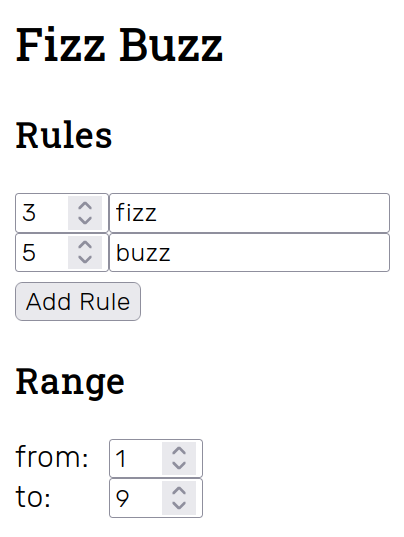
\includegraphics[width=.6\linewidth]{./mainmatter/pictures/fizzbuzz_control.png}
  \captionof{figure}{Fizz Buzz controls}
  \label{fig:fizzbuzz_control}
\end{minipage}%
\begin{minipage}{.5\textwidth}
  \centering
  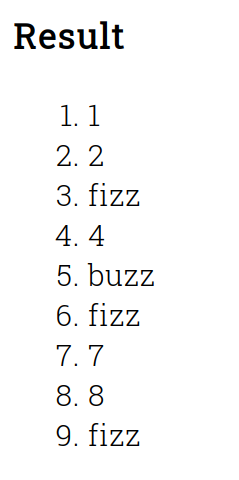
\includegraphics[width=.4\linewidth]{./mainmatter/pictures/fizzbuzz_result.png}
  \captionof{figure}{Fizz Buzz result}
  \label{fig:fizzbuzz_result}
\end{minipage}
\end{figure}

\subsection{JINQ}
\label{sub:results JINQ}
The following examples use |JINQ| to browse and process a JSON files.

\subsubsection{Find all Students}
\label{subsub:Find all Students}
We want to filter out all participants that have
a student ID. As you can see in the excerpt of the JSON file in
Listing~\ref{lst:json_file_devs}, the property |switch-edu-id| is
not defined for all persons. Because the |JsonMonad| works in the background with
|MaybeType|, such situations can be processed without null handling.

\begin{lstlisting}[
  style=json, 
  caption=Exerpt of a JSON File including developers,
  label={lst:json_file_devs}
  ]
[
  {
    "id": 1,
    "name": "",
    "age": 28,
    "salary": 50000,
    "favoriteLanguages": [1, 3, 5]
  },
  {
    "id": 2,
    "switch-edu-id": "12-432-23",
    "name": "Emma Johnson",
    "age": null,
    "salary": 60000,
    "favoriteLanguages": [2, 4]
  },
  {
    "id": 3,
    "name": "Sophia Davis",
    "age": 40,
    "salary": null,
    "favoriteLanguages": [null, 4, 5]
  },
  ...
 ]
\end{lstlisting}


\begin{lstlisting}[
  style=ES6, 
  caption=JINQ Example - find all students,
  label={lst:jinq_find_students}
  ]
const findAllStudentIds = developers => {
  const allIds =
    from(JsonMonad(developers))
      .select(x => x['switch-edu-id'])
      .result();
};
\end{lstlisting}

\subsubsection{Find Sophia's Programming Languages}
\label{subsub:Find Sophia's Programming Languages}

This example combines two JSON files. We use the JSON file from the previous
example and the one from Listing~\ref{lst:json_file_lang}.
Listing~\ref{lst:jinq_sophias_langs} shows the code that finds Sophia's 
favorite programming languages by combining two JSON files using |pairWith|. 

\begin{lstlisting}[
  style=json, 
  caption=Exerpt of a JSON File including programming languages,
  label={lst:json_file_lang}
  ]
[
  {
    "id": 1,
    "name": "Java"
  },
  ...
  {
    "id": 4,
    "name": "C++"
  },
  {
    "id": 5,
    "name": "Haskell"
  }
]
\end{lstlisting}

\begin{lstlisting}[
  style=ES6, 
  caption=JINQ example - find Sophia's programming languages,
  label={lst:jinq_sophias_langs}
  ]
const sophiasProgrammingLanguages = (devs, languages) =>
    from(JsonMonad(devs))
      .where   ( dev    => dev.name === "Sophia Davis")
      .select  ( sophia => sophia.favoriteLanguages)
      .pairWith( JsonMonad(languages) )
      .where   ( ([langId, language]) => langId === language.id )
      .select  ( ([     _, language]) => language.name )
      .result  ();
\end{lstlisting}

\subsection{Numerical Differentiation}
\label{sub:Numerical Differentiation}
This example shows a mathematical use case, the numberical differentiation using Sequences.

\begin{lstlisting}[
  style=ES6, 
  caption=Differentiation using Sequences,
  label={lst:diff_sequences}
  ]
const halve   = x => x / 2;
const repeatF = (f, x) => _.Sequence(x, _ => true, f);

const halves = h0 => repeatF( halve, h0);


const slope = f => x => h => (f(x + h) - f(x)) / h;

const differentiate = h0 => f => x => _.map ( slope(f)(x) ) (halves(h0));
\end{lstlisting}

Listing~\ref{lst:diff_sequences} implements the following steps: 


\begin{itemize}
  \item{|repeatF| repeatedly applies the function $f$ to a value of the
    previous calculated result, starting with $x$.}
  \item{ |halves| is using |repeatF| and |halve| to halve a value $h0$. With
      that, the value $h0$ is halved repearedly.} 
    \item{|slope| calculates the slope of a function $f$ at the position $x$
      with delta $h$.}
 \end{itemize}

We already have everything needed to be able to differentiate.  The function
differentiate calculates at a given point $x$ the slope more and more exactly.
Since this is an infinite Sequence, we have to define one more function.
Listing~\ref{lst:impl_within} shows the function |within|, which allows differentiating until a
given epsilon.

\begin{lstlisting}[
  style=ES6, 
  caption=Implementation of within,
  label={lst:impl_within}
  ]
const parabola = x => x * x;

const diffs = differentiate(0.5)(parabola)(1); *'\label{line:diffs}'*

const within = eps => sequence => {
  const [a, rest] = _.uncons(sequence);
  const [b]       = _.uncons(rest);
  const diff      = Math.abs(a - b);

  if (diff <= eps) return b;
  return within(eps)(rest);
};
const slopeOfFAtX = within(0.000_1)(diffs);
\end{lstlisting}

Listing~\ref{lst:impl_within} defines the following implementations:

\begin{itemize}
  \item{|parabola| is the function to work with in this example}
  \item{On line~\ref{line:diffs}, |diffs| defines a function to differentiate the |parabola| at point $1$ with
    starting value $h0$ of $0.5$.}
  \item{|within| calculates recursively the slope of the |parabola| using the
      sequence |diffs| until a satisfying accuracy. 
    \item{ At the end, |slopeOfFAtX| calculates the slope with the given parameters. }
    }
\end{itemize}


\subsection{Tic Tac Toe with a Kind of AI}
\label{sub:Alpha - Beta Algorithm}
This example includes the implementation of the alpha-beta heuristic, an
algorithm for games such as tic-tac-toe. The algorithm looks ahead to make the
optimal move. The implementation is adapted from the paper "Why Funcitonal
Programming Matters"~\cite{hughes_why_1989} to prove that even advanced 
applications in JavaScript can
be implemented using the Sequence library. For a deeper understanding of the
algorithm, you can either consult the paper mentioned before or the section
"Incremental Development" in Frege Goodness~\cite{frege_goodness}.

\subsubsection{The Required Types}
\label{subsub:The Required Types}
Listing~\ref{lst:tictactoe_types} shows the required types for the game
implementation.

\begin{lstlisting}[
  style=ES6, 
  caption=Tic Tac Toe Types,
  label={lst:tictactoe_types}
  ]
/**
 * @template _T_
 * @typedef {SequenceType<Tree<_T_>>} TreeSequence
 */

/**
 * @template _T_
 * @typedef { PairSelectorType<_T_, TreeSequence<_T_>> } Tree
 */


/**
 * @typedef { "Computer" | "Human" | "NoPlayer" } Player
 */

/**
 * @typedef { 1 | -1 | 0 } Stone
 */

/**
 * @typedef Board
 * @property { Player } whosTurn
 * @property { Iterable<Stone>} fields - A board has fields from 0 to 8.
 */
\end{lstlisting}

Listing~\ref{lst:tictactoe_players} includes the definition of the players and some
functions used in the game process. Since JavaScript does not support pattern
matching, the functions |opponent| and |stone| use a workaround via an object.

\begin{lstlisting}[
  style=ES6, 
  caption=The players and some helper functions,
  label={lst:tictactoe_players}
  ]
/** @type { Player } */
const Computer = "Computer";

/** @type { Player } */
const Human = "Human";

/** @type { Player } */
const NoPlayer = "NoPlayer";

/**
 * Returns the opponent of a given player.
 * @param { Player } player
 * @return Player
 */
const opponent = player => {
  const pairings = {
    "Computer" : Human,
    "Human"    : Computer,
    "NoPlayer" : NoPlayer,
  };
  return pairings[player];
};

/**
 * Returns the stone number of a given player.
 * @param { Player } player
 * @returns Stone
 */
const stone = player => {
  const pairings = {
    "Computer" :  1,
    "Human"    : -1,
    "NoPlayer" :  0,
  };
 return pairings[player];
};

/**
 * Transforms each board element using the given function f.
 * @template _T_, _U_
 * @type {
 *         (f: (Board) => _T_)
 *      => (tree: Tree<_U_>)
 *      => Tree<_T_>
 * }
 */
const treeMap = f => ([a, sub]) => Pair(f(a))(map(treeMap(f))(sub));
\end{lstlisting}

\subsubsection{Processing the Game Board}
\label{subsub:Processing the Game Board}

Listing~\ref{lst:tictactoe_move} includes the |moves| function. This function
calculates all possible moves for a player whose turn it is on the board.
\begin{lstlisting}[
  style=ES6, 
  caption=Tic Tac Toe move function,
  label={lst:tictactoe_move}
  ]
/**
 * Indexes each field using a {@link PairType}.
 * @param { Iterable<Stone> } fields
 * @return { SequenceType<PairType<Stone, Number>> }
 */
const indexFields = fields => zip(fields)(Range(1,9));

/**
 * Calculates possible moves for a given board.
 * @param { Board } board
 * @return SequenceType<Board>
 */
const moves = board => {
  if (hasWon(board)(Computer)) return /**@type {SequenceType<Board>} */nil;
  if (hasWon(board)(Human))    return /**@type {SequenceType<Board>} */nil;
  const otherPlayer = opponent(board.whosTurn);

  const indexedFields = indexFields(board.fields);

  const blankIndices =
    from(indexedFields)
      .where( ([content, _]) => content === stone(NoPlayer))
      .select( ([_, i]) => i)
      .result();

  const fieldsWithPlayerPlacedAt = pos =>
    from(indexedFields)
      .select(([content, i]) => i === pos ? stone(board.whosTurn) : content)
      .result();

  const boardFieldsAfterMove = map(fieldsWithPlayerPlacedAt)(blankIndices);

  return /** @type SequenceType<Board> */ 
       map(fields => ({fields, whosTurn: otherPlayer}))(boardFieldsAfterMove);
}
\end{lstlisting}

Listing~\ref{lst:tictactoe_hasWon} shows the implementation of the |hasWon|
function, which checks if a player has won on a given board.
\begin{lstlisting}[
  style=ES6, 
  caption=Tic Tac Toe hasWon function,
  label={lst:tictactoe_hasWon}
  ]
/**
 * Checks, if a player has won.
 * @type {
 *    (board: Board)
 *    => (player: Player)
 *    => Boolean
 * }
 */
const hasWon = board => player => {
  const winTriples = [
    [1,2,3], [4,5,6], [7,8,9], // row
    [1,4,7], [2,5,8], [3,6,9], // col
    [1,5,9], [3,5,7]           // diag
  ];

  const checkTriple = triple => {
    const actualStone = stone(player);
    const indexedFields = indexFields(board.fields);

    const playerOnFields =
      from(indexedFields)
      .where( ([_, i])        => triple.includes(i))
      .select( ([content, _]) => content === actualStone)
      .result();

    return foldl$((acc, cur) => acc && cur, true)(playerOnFields);
  };
  return pipe(
    map(checkTriple),
    foldl$((acc, cur) => acc || cur, false)
  )(winTriples)
};
\end{lstlisting}


Listing~\ref{lst:tictactoe_gametree} shows the functions to build a game tree.
\begin{lstlisting}[
  style=ES6, 
  caption=Tic Tac Toe game tree,
  label={lst:tictactoe_gametree}
  ]
/**
 * Generates recursively a game tree, which is potentially endless.
 * @template _T_
 * @type {
 *       (unfold: ((_T_) => Iterable<_T_>))
 *    => (a: _T_)
 *    => Tree<_T_>
 * }
 */
const buildTree = unfold => a => {
  const as = unfold(a);
  const children = map(buildTree(unfold))(as);
  return Pair(a)(children);
};

/**
 * Creates a game tree.
 * @param { Board } board
 * @returns Tree<Board>
 */
const gameTree = board => buildTree(moves)(board);
\end{lstlisting}

\subsubsection{The Minimax Algorithm}
\label{subsub:minimax_algo}
Listing~\ref{lst:tictactoe_minimax} shows the implementation of the Minimax
algorithm. These functions determine which are the best moves.
\begin{lstlisting}[
  style=ES6, 
  caption=Tic Tac Toe minimax algorithmus,
  label={lst:tictactoe_minimax}
  ]
/**
 * Evaluates a given board.
 * @param { Board } board
 * @returns Number
 */
const staticEval = board => {
  if (hasWon(board)(Computer)) return  1.0;
  if (hasWon(board)(Human))    return -1.0;
  return 0.0;
};

/**
 * Determines the best move.
 * @template _T_
 * @param { Tree<_T_>}
 * @return { _T_ }
 */
const maximize = ([a, sub]) => {
  if (sub ["=="] (nil)) return a;
  return max$ (map(minimize)(sub))
};

/**
 * Determines the best move for the opponent.
 * @template _T_
 * @param { Tree<_T_>}
 * @return { _T_ }
 */
const minimize = ([a, sub]) => {
  if (sub ["=="] (nil)) return a;
  return min$ (map(maximize)(sub))
};
\end{lstlisting}

\subsubsection{Pruning a Game Tree}
\label{subsub:Pruning a Game Tree}

We must prune the game tree for a specific calculation since we are dealing with
potentially endless trees. The following Listing~\ref{lst:tictactoe_prune} shows
the implementation.

\begin{lstlisting}[
  style=ES6, 
  caption=Tic Tac Toe prune function,
  label={lst:tictactoe_prune}
  ]
/**
 * Prunes a given {@link Tree} to a max depth n.
 * @template _T_
 * @type {
 *           (n: Number)
 *        => (tree: Tree<_T_>)
 *        => Tree<_T_>
 * }
 * @param n
 */
const prune = n => tree => {
  const [a, sub] = tree;
  if (n === 0) return Pair(a)(nil);
  else return Pair(a)(map(prune(n-1))(sub));
};
\end{lstlisting}

\subsubsection{The Evaluation}
\label{subsub:The Evaluation}

The following functions evaluate a game board. The function |nextBoardBy|
calculates the next move for the computer based on the number of lookaheads,
i.e., how many moves are calculated ahead.

\begin{lstlisting}[
  style=ES6, 
  caption=Tic Tac Toe - evaluating functions,
  label={lst:tictactoe_eval}
  ]
/**
 * Evaluating a board with a max number of lookaheads.
 * @template _T_
 * @type {
 *            (f: (Board) => _T_)
 *         => (lookahead: Number)
 *         => (board: Board)
 *         => _T_
 * }
 */
const evaluateBy = f => lookahead => board => {
  const prunedTree = prune(lookahead)(gameTree(board));
  const mappedTree = treeMap(f)(prunedTree);
  return minimize(mappedTree);
};

/**
 * @template _T_
 * @type {
 *            (lookahead: Number)
 *         => (board: Board)
 *         => PairSelectorType<_T_, Board>
 * }
 */
const nowValue = lookahead => board =>
  Pair(evaluateBy(staticEval)(lookahead)(board))(board);

/**
 * Calculates the next board with given board fields.
 * @type {
 *          (lookahead: Number)
 *       => (inFields: Array<Number>)
 *       => Board
 * }
 */
const nextBoardBy = lookahead => inFields => {
  const possibleMoves  = moves ({whosTurn: Computer, fields: inFields});
  const evaluatedMoves = 
      /** @type {SequenceType<PairSelectorType<Number, Board>>} */ 
      map (nowValue(lookahead)) (possibleMoves);


  /**
   *
   * @param { SequenceType<PairSelectorType<Number, Board>> } boards
   * @return Board
   */
  const bestOf = boards => {
    if (isEmpty(boards)) return {whosTurn: NoPlayer, fields: []};
    return max$(boards, ([a, _b1],[b, _b2]) => a < b )(snd);
  };
  return bestOf(evaluatedMoves);
};
\end{lstlisting}


